\section{Class Diagram}\label{sec:class-diagram}
The class diagram in Figure~\ref{fig:class-diagram} shows the relationships between the different classes in the system.
The \texttt{Model} class represents the underlying model of the system, which can be a CTMC, DTMC, HMM and MDP.
The \texttt{Model} class has a aggregation relationship with the \texttt{Algorithm} class, which represents the functions used in the Baum-Welch algorithm, with and without ussing log-semiring.
The \texttt{Algorithm} class has a dependency relationship with the \texttt{CUDD} class, which is a wrapper for the CUDD library.
The \texttt{CUDD} class is used to perform the matrix operations as ADD's required by the Baum-Welch algorithm.
The \texttt{Model} class also has a aggregation relationship with the \texttt{CUDD} class, as the \texttt{Model} class uses the \texttt{CUDD} class to perform the ADD operations.

\subsection{\texttt{Model} Class}
The \texttt{Model} class serves as the foundation for representing various probabilistic models like CTMC, MDP, and DTMC. 
It holds fields needed to describe these models, such as the transition matrices, emission probabilities, and initial states, all represented using Algebraic Decision Diagrams (ADDs). 
The \texttt{Model} class also provides methods for training models, such as the Baum-Welch algorithm.

\textbf{Attributes:}
\begin{itemize}
    \item \texttt{Type\_model}: Defines the type of model (e.g., CTMC, MDP, DTMC).
    \item \texttt{transfer}: A list of ADD structures representing state transition probabilities.
    \item \texttt{Emission}: An ADD for the emission probabilities (relevant in Hidden Markov Models).
    \item \texttt{pi}: The initial state distribution, also stored as an ADD.
    \item \texttt{training\_set}: A collection of observed data.
\end{itemize}
\textbf{Methods:}
\begin{itemize}
    \item \texttt{Instantiate\_with\_parameters(prismfile, parameters: Dictionary)}: Instantiates a model with specified parameters.
    \item \texttt{Instantiate\_without\_parameters(prismfile)}: Creates a model without additional parameters.
    \item \texttt{Baum-welsh(log, Model)}: This method implements the Baum-Welch algorithm for training Hidden Markov Models, utilizing various operations from the \texttt{Algorithm} class.
\end{itemize}

\subsection{\texttt{CUDD} Class}
The \texttt{CUDD} class (CUDD Manager) is responsible for managing ADDs. These ADDs are crucial in representing the probabilistic data structures used in the \texttt{Model} class. \texttt{CUDD} provides a set of operations that allow mathematical and logical manipulation of these diagrams.

\textbf{Attributes:}
\begin{itemize}
    \item \texttt{rowvars, colvars}: Representing variables used in the ADD structures.
    \item \texttt{ADD}: The main data structure for storing probabilities or logical expressions.
    \item \texttt{Manager}: A control structure that coordinates operations on ADDs.
\end{itemize}
\textbf{Methods:}
\begin{itemize}
    \item \texttt{Hadamard(), Log\_Hadamard()}: Perform element-wise operations on ADDs.
    \item \texttt{Matrix\_mul(), Log\_matrix\_mul()}: For matrix multiplications.
    \item \texttt{Sum(), Transpose()}: Additional helper methods for summing and transposing ADDs.
\end{itemize}

\subsection{\texttt{Algorithm} Class}
The \texttt{Algorithm} class encapsulates various methods for performing probabilistic calculations. These methods are mainly used for inference in models such as Hidden Markov Models (HMM) and Markov Chains.

\textbf{Methods:}
\begin{itemize}
    \item \texttt{calculate\_alpha(), calculate\_beta()}: Compute the forward (alpha) and backward (beta) probabilities, respectively.
    \item \texttt{calculate\_gamma(), calculate\_xi()}: Intermediate probability calculations needed for parameter estimation and model training.
\end{itemize}
Each method operates on the ADD structures created and managed by the \texttt{CUDD} class, ensuring efficient computation of the probabilities.

\subsection{Relationships Between Classes}
\subsubsection{\texttt{Model} to \texttt{Algorithm}: Association Relationship}
The \texttt{Model} class uses the \texttt{Algorithm} class to compute the forward-backward probabilities and other values necessary for inference. 
The Baum-welsh(log, Model) method in \texttt{Model} invokes the relevant methods from \texttt{Algorithm} (calculate\_alpha(), calculate\_beta(), etc.) during the training process of HMMs. 
These methods, while called collectively in Baum-Welch, can also be used independently to perform specific calculations.

\subsubsection{\texttt{Model} to \texttt{CUDD}: Aggregation Relationship}
The \texttt{Model} class contains several attributes (transfer, Emission, pi) that are represented as ADDs, managed by the \texttt{CUDD} class.
This relationship is best represented as an aggregation, where the \texttt{Model} holds instances of ADD but does not directly manage their internal workings.
Instead, \texttt{CUDD} provides the operations required to manipulate and operate on these diagrams, such as matrix multiplication or element-wise functions (Hadamard products).
The \texttt{Model} depends on \texttt{CUDD} for these operations, making it an integral part of the system's backend.

\subsubsection{\texttt{Algorithm} to \texttt{CUDD}: Dependency Relationship}
The \texttt{Algorithm} class depends on the \texttt{CUDD} class for all its operations on ADDs.
Every method in \texttt{Algorithm} (e.g., calculate\_alpha(), calculate\_gamma()) relies on ADD operations provided by \texttt{CUDD}, such as Matrix\_mul() and Hadamard().
This is represented by a dependency relationship, where \texttt{Algorithm} calls \texttt{CUDD}'s methods to perform its computations.

\begin{figure}
    \centering
    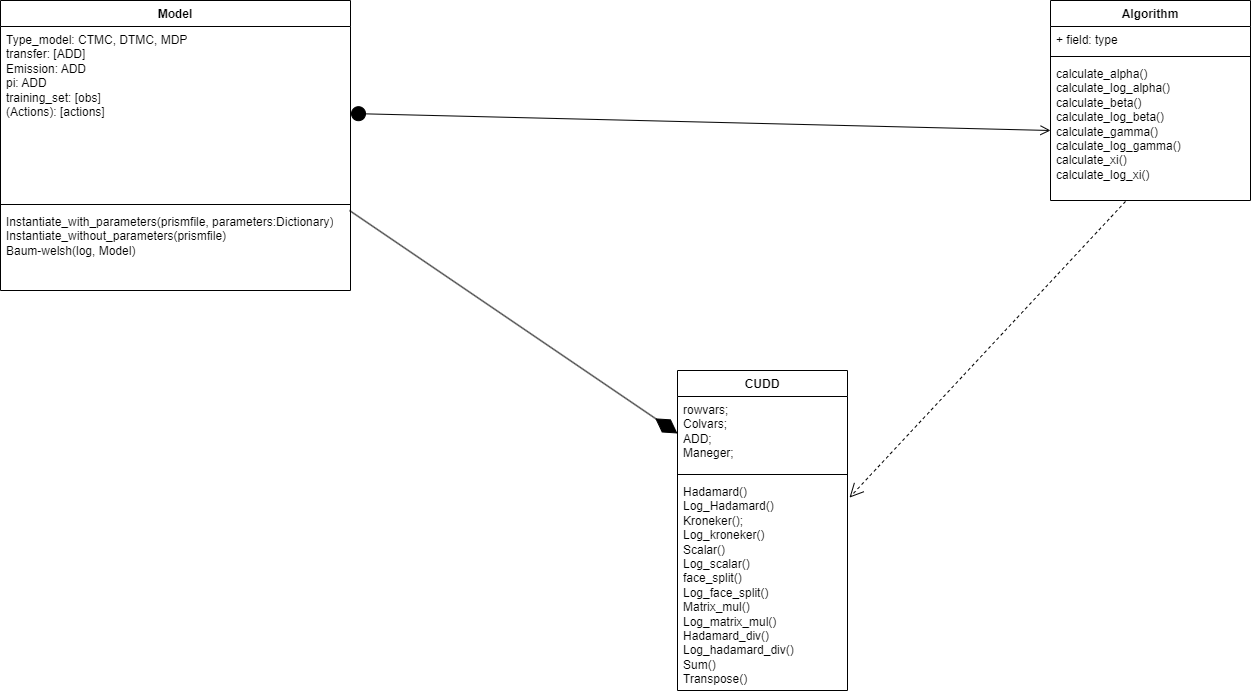
\includegraphics[width=0.5\textwidth]{figures/class-diagram.png}
    \caption{Class diagram of the system}
    \label{fig:class-diagram}
\end{figure}